% Draft (2026-11-10). One-page architecture figure for the Week 08 midterm.
% Build: pdflatex architecture.tex  (needs TeX Live with tikz + kotex, or xelatex with a Korean font)
\documentclass[tikz,border=8pt]{standalone}
\usetikzlibrary{positioning,arrows.meta,fit,backgrounds}
\begin{document}
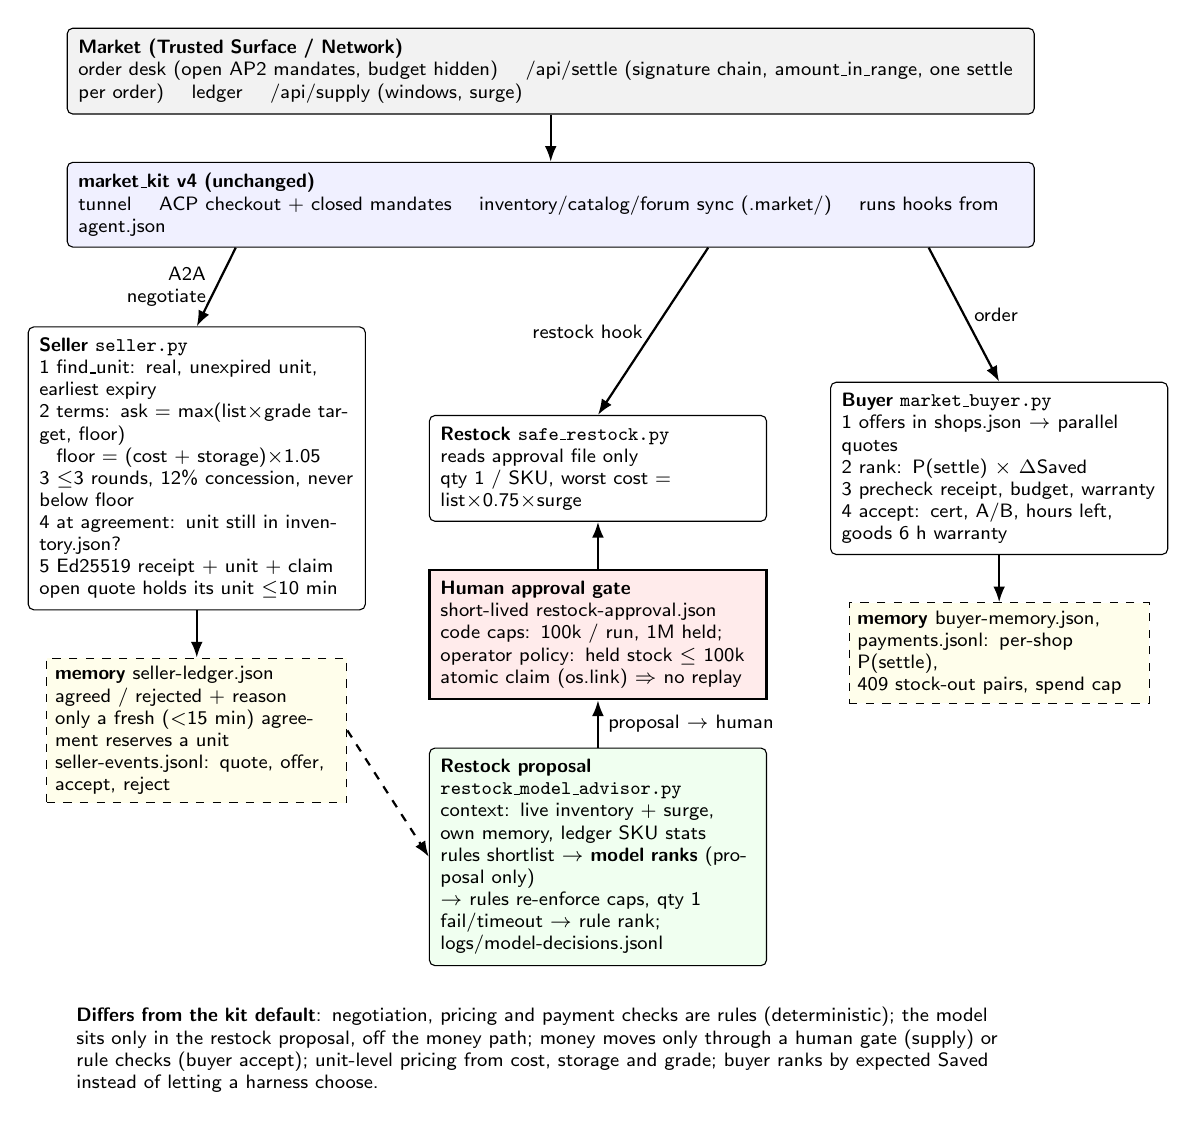
\begin{tikzpicture}[
  font=\sffamily\scriptsize, node distance=6mm and 8mm,
  box/.style={draw, rounded corners=2pt, align=left, inner sep=4pt, text width=#1},
  box/.default=40mm,
  mem/.style={draw, dashed, align=left, inner sep=3pt, text width=36mm, fill=yellow!8},
  gate/.style={draw, thick, fill=red!8, align=left, inner sep=4pt, text width=40mm},
  arr/.style={-{Latex[length=2mm]}, thick},
  grp/.style={draw, rounded corners=4pt, inner sep=6pt, fill=#1},
]
% ---------------- Market ----------------
\node[box=120mm, fill=gray!10] (market) {\textbf{Market (Trusted Surface / Network)}\\
order desk (open AP2 mandates, budget hidden) \quad /api/settle (signature chain, amount\_in\_range, one settle per order) \quad ledger \quad /api/supply (windows, surge)};

% ---------------- Kit ----------------
\node[box=120mm, fill=blue!6, below=of market] (kit) {\textbf{market\_kit v4 (unchanged)}\\
tunnel \quad ACP checkout + closed mandates \quad inventory/catalog/forum sync (.market/) \quad runs hooks from agent.json};

% ---------------- Seller column ----------------
\node[box, below left=10mm and -38mm of kit] (seller) {\textbf{Seller} \texttt{seller.py}\\
1 find\_unit: real, unexpired unit, earliest expiry\\
2 terms: ask = max(list$\times$grade target, floor)\\
\phantom{2 }floor = (cost + storage)$\times$1.05\\
3 $\le$3 rounds, 12\% concession, never below floor\\
4 at agreement: unit still in inventory.json?\\
5 Ed25519 receipt + unit + claim\\
open quote holds its unit $\le$10 min};
\node[mem, below=of seller] (sl) {\textbf{memory} seller-ledger.json\\agreed / rejected + reason\\only a fresh ($<$15 min) agreement reserves a unit\\seller-events.jsonl: quote, offer, accept, reject};

\node[box, right=of seller] (restock) {\textbf{Restock} \texttt{safe\_restock.py}\\
reads approval file only\\ qty 1 / SKU, worst cost = list$\times$0.75$\times$surge};
\node[gate, below=of restock] (approve) {\textbf{Human approval gate}\\
short-lived restock-approval.json\\code caps: 100k / run, 1M held;\\operator policy: held stock $\le$ 100k\\atomic claim (os.link) $\Rightarrow$ no replay};
\node[box, fill=green!6, below=of approve] (analysis) {\textbf{Restock proposal} \texttt{restock\_model\_advisor.py}\\
context: live inventory + surge, own memory, ledger SKU stats\\
rules shortlist $\rightarrow$ \textbf{model ranks} (proposal only)\\
$\rightarrow$ rules re-enforce caps, qty 1\\
fail/timeout $\rightarrow$ rule rank; logs/model-decisions.jsonl};

% ---------------- Buyer column ----------------
\node[box, right=of restock] (buyer) {\textbf{Buyer} \texttt{market\_buyer.py}\\
1 offers in shops.json $\rightarrow$ parallel quotes\\
2 rank: P(settle) $\times$ $\Delta$Saved\\
3 precheck receipt, budget, warranty\\
4 accept: cert, A/B, hours left, goods 6 h warranty};
\node[mem, below=of buyer] (bm) {\textbf{memory} buyer-memory.json,\\payments.jsonl: per-shop P(settle),\\409 stock-out pairs, spend cap};

% ---------------- arrows ----------------
\draw[arr] (market) -- (kit);
\draw[arr] (kit.south) ++(-40mm,0) -- node[left,align=right]{A2A\\negotiate} (seller.north);
\draw[arr] (kit.south) ++(20mm,0) -- node[left]{restock hook} (restock.north);
\draw[arr] (kit.south) ++(48mm,0) -- node[right]{order} (buyer.north);
\draw[arr] (seller) -- (sl);
\draw[arr] (buyer) -- (bm);
\draw[arr] (approve) -- (restock);
\draw[arr] (analysis) -- node[right]{proposal $\rightarrow$ human} (approve);
\draw[arr, dashed] (sl.east) -- (analysis.west);

\node[align=left, text width=120mm, below=4mm of analysis.south west, anchor=north west, xshift=-46mm] {
\textbf{Differs from the kit default}: negotiation, pricing and payment checks are rules (deterministic); the model sits only in the restock proposal, off the money path; money moves only through a human gate (supply) or rule checks (buyer accept); unit-level pricing from cost, storage and grade; buyer ranks by expected Saved instead of letting a harness choose.};
\end{tikzpicture}
\end{document}
